\section{Quantum Modular Exponentiation}
\label{sec:modexp}

We now extend our arithmetic to modular exponentiation, which is repeated
modular multiplication controlled on qubits supplied by a phase estimation
procedure.
If we wish to multiply an $n$-qubit quantum input number $\ket{x}$ by
$t$ classical numbers $a^{(j)}$, we can multiply them in series.
% as shown in
%Figure \ref{fig:modexp-qc-series}.
This requires depth $O(t\log n)$ in modular multiplication operations.

%\begin{figure}[htp!]
%\begin{center}
%\includegraphics[width=5.5in]{figures/modexp-qc-series.pdf}
%\end{center}
%\caption{Multiplying a quantum number $\ket{x}$ by $t$ classical numbers
%$\{a^{0}, a^{1}, \ldots, a^{n-1}\}$ in series.}
%\label{fig:modexp-qc-series}
%\end{figure}

Now consider the same procedure, but this time each classical number $a^{(j)}$
is controlled on a quantum bit $p_j$. This is a special case of
multiplying by $t$ quantum integers in series, since a classical number
entangled with a quantum integer is also quantum.
%This is shown in
%Figure \ref{fig:modexp-qq-series}.
It takes the same depth $O(t\log n)$ as the previous case.
%
%\begin{figure}[htp!]
%\begin{center}
%\includegraphics[width=5.5in]{figures/modexp-qq-series.pdf}
%\end{center}
%\caption{Multiplying a quantum number $\ket{x}$ by $t$ quantum numbers
%$\{\ket{a^{0}p_0}, \ket{a^{1}p_1}, \ldots, \ket{a^{n-1}p_{n-1}}\}$ in series.}
%\label{fig:modexp-qq-series}
%\end{figure}

Finally, we consider multiplying $t$ quantum integers
$\{x^{(1)}, x^{(2)}, \ldots, x^{(t-1)}, x^{(t)}\}$ in a parallel,
logarithmic-depth binary tree.
This is shown in Figure \ref{fig:modexp-qq-parallel}, where arrows indicate multiplication.
The tree has depth $\log_2(t)$ in modular multiplier operations. Furthermore,
each
modular multiplier has depth $O(\log(n))$ and width $O(n^3)$ for $n$-qubit
numbers. Therefore, the overall depth of this parallel modular exponentiation
structure is $O(\log(t)\log(n))$ with width $O(tn^3)$.
In phase estimation for QPF, it is
sufficient to take $t = O(n)$ \cite{Nielsen2000,Kitaev2002}. Therefore our total depth is
$O(\log^2(n))$ and our total size and total width are $O(n^4)$, as desired. At this point, combined with the parallel phase
estimation procedure of \cite{Kitaev2002}, we have a complete factoring
implementation in our 2D nearest-neighbor architecture in polylogarithmic
depth.
%
\begin{figure*}[tb!]
\centerline{
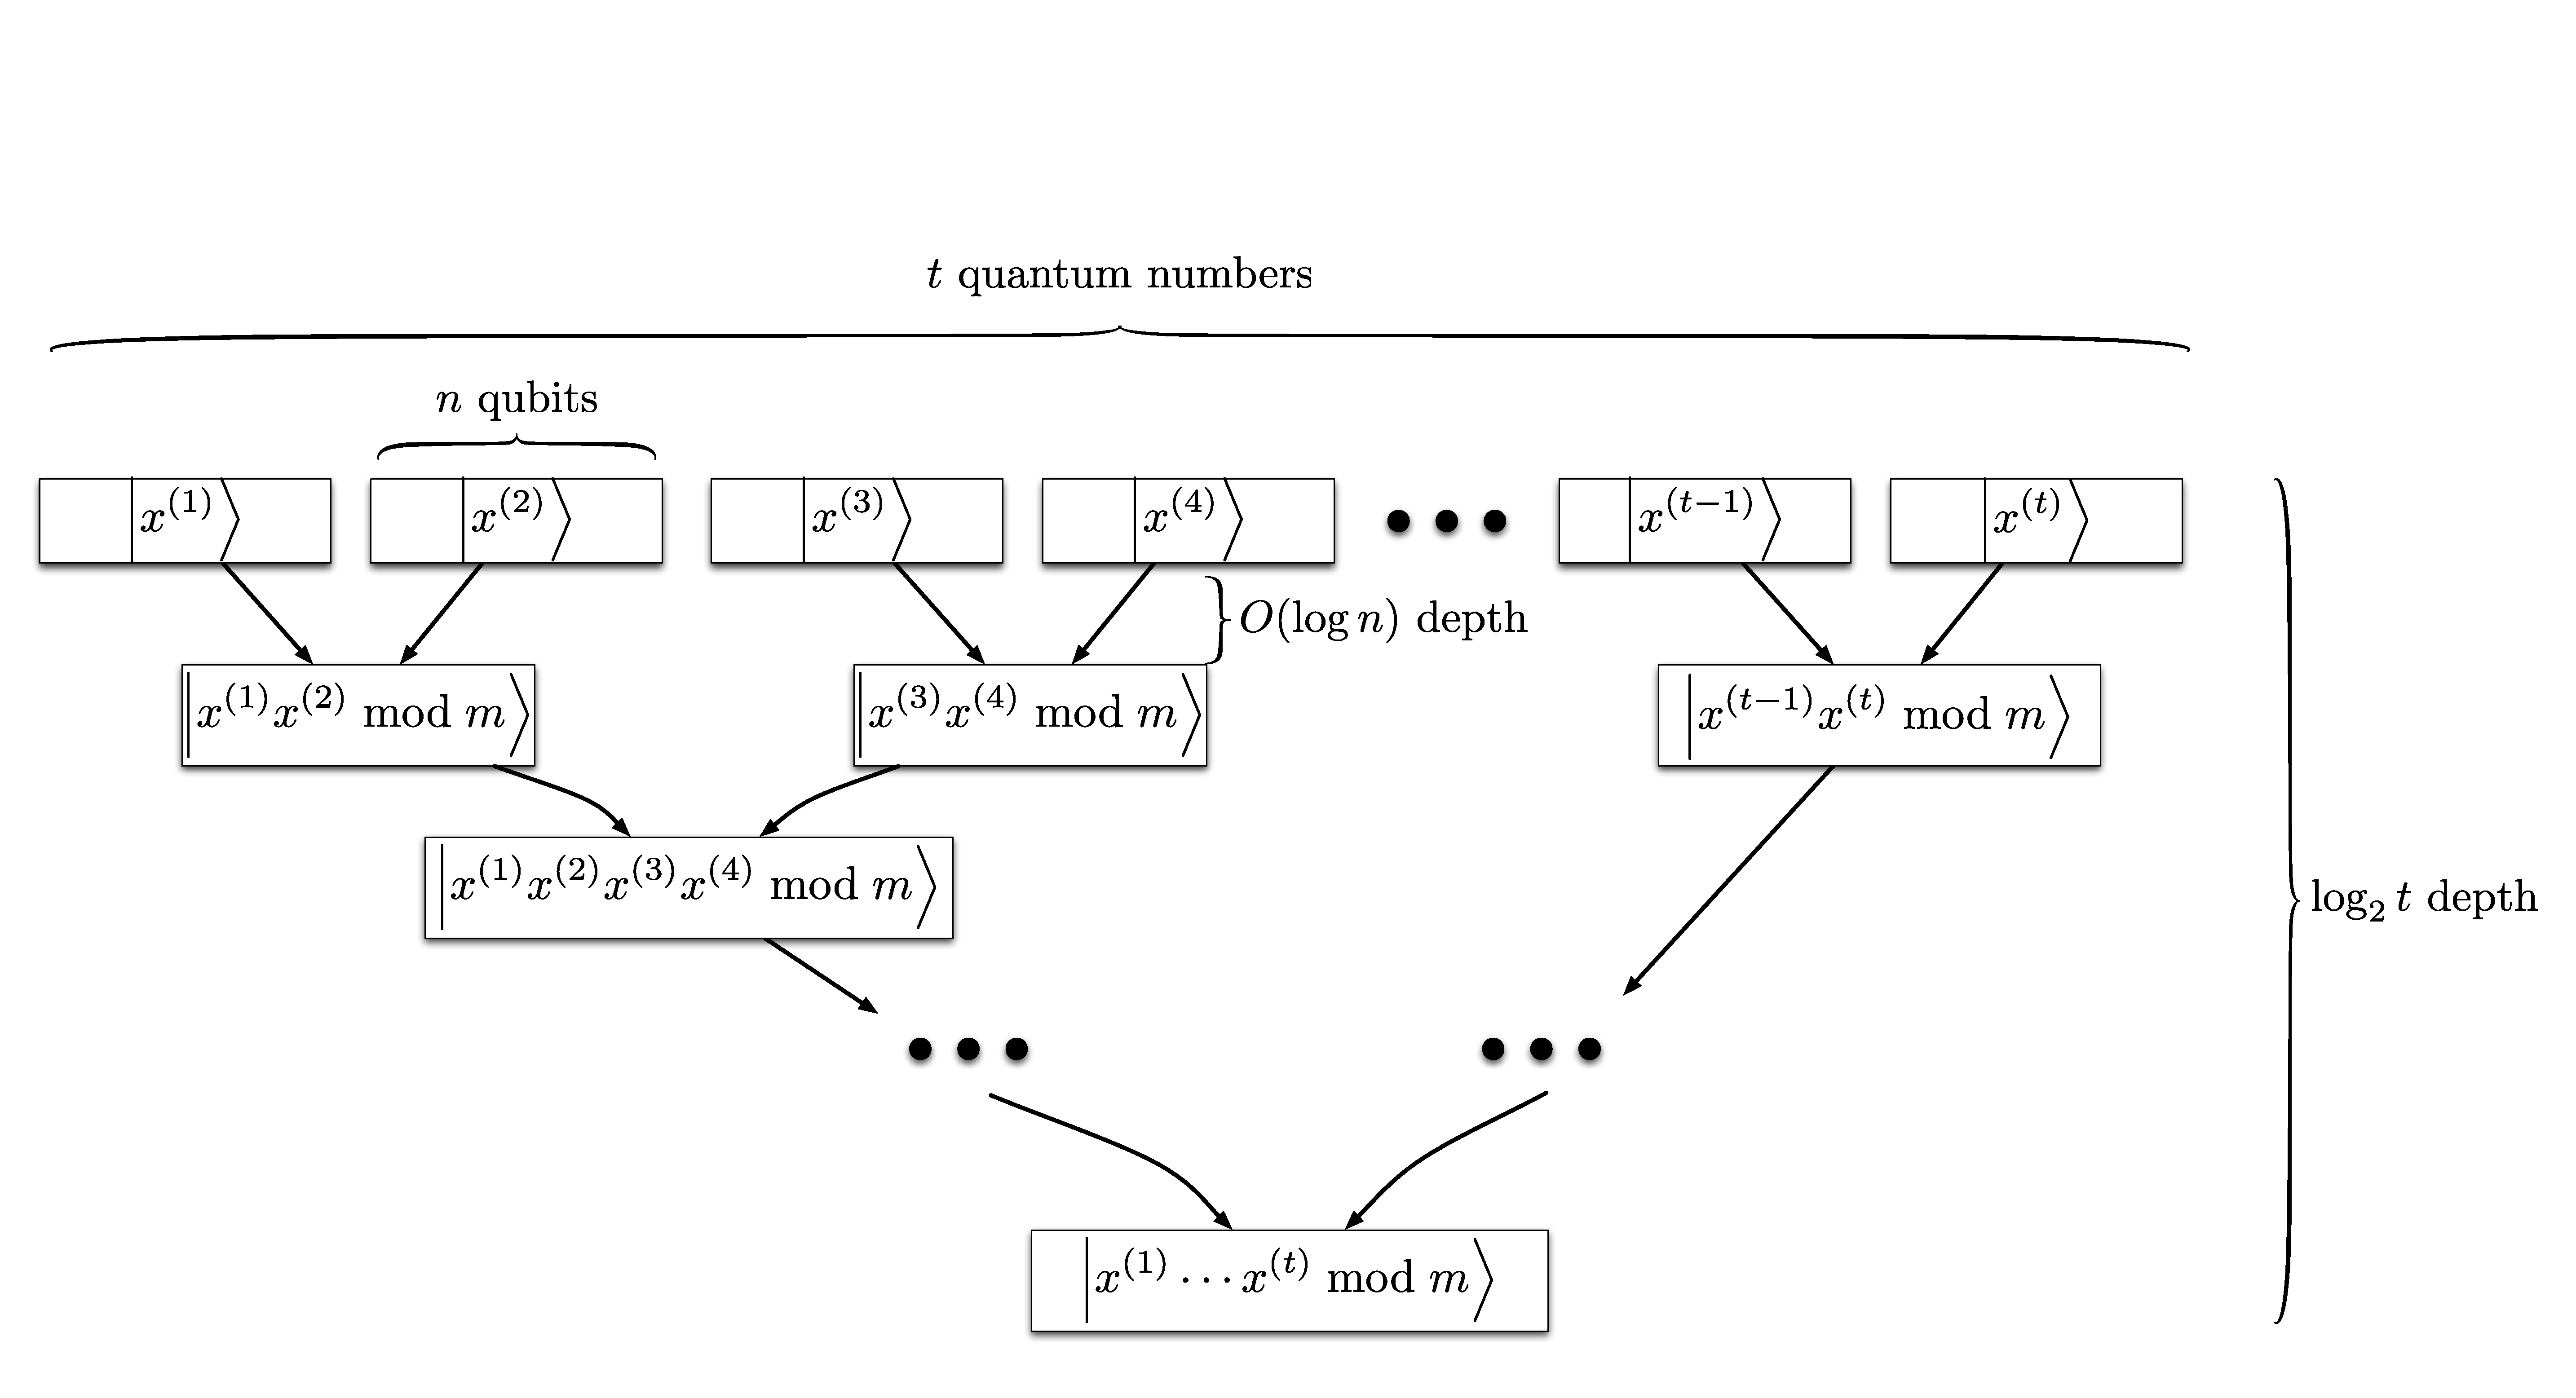
\includegraphics[width=5.5in]{./mod-exp-par.pdf}
}
\fcaption{Parallel modular exponentiation: multiplying $t$ quantum integers
%$\{\ket{x^{(0)}}, \ket{x^{(1)}}, \ldots, \ket{x^{(t-1)}}\}$ in parallel,
in a $O(\log{(t)}\log{(n)})$-depth binary tree. Arrows indicate modular
multiplication.}
\label{fig:modexp-qq-parallel}
\end{figure*}

We will now calculate numerical
constants to upper bound circuit resources.

According to the Kitaev-Shen-Vyalyi parallelized phase estimation procedure
\cite{Kitaev2002},
for a constant success probability of $3/4$,
it is sufficient to multiply together $t' = 2867n$ quantum integers,
controlled on the qubits $\ket{p_j}$, in parallel.

In Section \ref{subsec:qcla}, we describe the last step of modular
exponentiation in CSE. In Section \ref{subsec:modexp-resources}, we
state the final circuit resources for the entire modular exponentiation
circuit,
and therefore, our quantum period-finding procedure.

%%%%%%%%%%%%%%%%%%%%%%%%%%%%%%%%%%%%%%%%%%%%%%%%%%%%%%%%%%%%%%%%%%%%%%%%%%%%%%
\subsection{Converting Back to a Unique Conventional Number}
\label{subsec:qcla}

The final product of all $t$ quantum integers is in CSE which is not
unique. As stated in Gossett's original paper \cite{Gossett1998}, this
must be converted back to a conventional number using, for example, the
quantum carry-lookahead adder (QCLA) from \cite{Draper2004}. We can convert
this to a nearest-neighbor architecture by using the qubit reordering
construction of \cite{Rosenbaum2012}. We now compute the resources
needed for this last step.

To add two $(n+2)$-bit numbers in a QCLA, we have a circuit width of
$k = (4(n+2) - 2\log_2 n - 1)$. The depth is at most $4\log_2 n +2$ gates,
and some of them act on qubits that are not nearest-neighbors. Therefore,
we add in between each gate a reordering circuit that takes $k^2$
(reusable) ancillae
qubits and uses two rounds of constant-depth teleportation to rearrange
the qubits into a new order where all the gates are nearest-neighbor.
Adding in the teleportation circuit resources from Table \ref{tab:cd-resources},
we can calculate the following resources.

The circuit depth is $O(\log n)$:

\begin{equation}
56\log_2 n + 28\text{.}
\end{equation}

The circuit size is $O(n^2 \log n)$:

\begin{eqnarray}
96 \log_2^3 n & - & (384n + 624)\log_2^2 n \nonumber \\
              & + & (384n^2 + 1152n + 840) \log_2 n \nonumber \\
              & + & (192n^2 + 672n + 588)\text{.}
\end{eqnarray}

The circuit width is $O(n^2)$:

\begin{equation}
4 \log_2^2 n - (16n + 30)\log_2 n + 16n^2 + 60n + 56\text{.}
\end{equation}


%%%%%%%%%%%%%%%%%%%%%%%%%%%%%%%%%%%%%%%%%%%%%%%%%%%%%%%%%%%%%%%%%%%%%%%%%%%%%%
\subsection{Circuit Resources for Modular Exponentiator}
\label{subsec:modexp-resources}

This leads to the following circuit resource upper bounds for a modular exponentiator. Therefore, these are the total resources for running a
single round of parallel QPF as part of Shor's factoring algorithm.

The circuit depth is $O(\log^2 n)$:

% From Notebook #16 p. 225
\begin{equation}
D_{ME} = 1383\log_2^2(n) + 21253\log_2(n) + 49095\text{.}
\end{equation}

The module depth is $O(\log n)$:

\begin{equation}
\overline{D}_{ME} = 3\log_2 n + 24
\end{equation}

The circuit size is $O(n^4)$:

\begin{eqnarray}
S_{ME} & = & 96 \log_2^3 n + \nonumber \\
       & - & (384n + 624)\log_2^2 n \nonumber \\
       & + & (384n^2 + 1152n + 840) \log_2 n \nonumber \\
       &   & 3302324 n^4 + 30900797 n^3 + 50521837 n^2  + 20284306 n + 
  -6494\text{.}
\end{eqnarray}

The module size is $O(n^2)$:

\begin{equation}
\overline{S}_{ME} = 5749n^2 + 8725n +175\text{.}
\end{equation}

The circuit width is $O(n^4)$:

\begin{equation}
W_{ME} = 94598n^4 + 799749 n^3 + 1246692 n^2 + 415222 n - 145\text{.}
\end{equation}

The module width is $O(n)$:

\begin{equation}
\overline{W}_{ME} = 1434n\text{.}
\end{equation}